\documentclass[12pt]{article}
\setlength\parindent{0pt}
\usepackage{fullpage}
\usepackage{epsf}
\usepackage{amsmath}
\usepackage{graphicx}
\setlength{\parskip}{4mm}
\def\LL{\left\langle}   % left angle bracket
\def\RR{\right\rangle}  % right angle bracket
\def\LP{\left(}         % left parenthesis
\def\RP{\right)}        % right parenthesis
\def\LB{\left\{}        % left curly bracket
\def\RB{\right\}}       % right curly bracket
\def\PAR#1#2{ {{\partial #1}\over{\partial #2}} }
\def\PARTWO#1#2{ {{\partial^2 #1}\over{\partial #2}^2} }
\def\PARTWOMIX#1#2#3{ {{\partial^2 #1}\over{\partial #2 \partial #3}} }
\newcommand{\BE}{\begin{displaymath}}
\newcommand{\EE}{\end{displaymath}}
\newcommand{\BNE}{\begin{equation}}
\newcommand{\ENE}{\end{equation}}
\newcommand{\BEA}{\begin{eqnarray}}
\newcommand{\EEA}{\nonumber\end{eqnarray}}
\newcommand{\EL}{\nonumber\\}
\newcommand{\la}[1]{\label{#1}}
\newcommand{\ie}{{\em i.e.\ }}
\newcommand{\eg}{{\em e.\,g.\ }}
\newcommand{\cf}{cf.\ }
\newcommand{\etc}{etc.\ }
\newcommand{\Tr}{{\rm tr}}
\newcommand{\etal}{{\it et al.}}
\newcommand{\OL}[1]{\overline{#1}\ } % overline
\newcommand{\OLL}[1]{\overline{\overline{#1}}\ } % double overline
\newcommand{\OON}{\frac{1}{N}} % "one over N"
\newcommand{\OOX}[1]{\frac{1}{#1}} % "one over X"



\begin{document}
\pagenumbering{gobble}
\begin{center}
\Large\sc{Diagnostic Quiz: Taylor Series}

\normalsize\it
This quiz will not be graded. I am giving it to you only as a diagnostic, so I can learn what you already know about Taylor series, and to guide the teaching of this class and the design of the physics curriculum. 
\end{center}



\begin{enumerate}

\item{Have you studied Taylor series (perhaps called ``power series'' or ``Maclaurin series'') in a mathematics class?}
\vspace{1in}

\item{Have you studied Taylor series in a physics or engineering class, such as mathematical methods?}
\vspace{1in}

\item{In what physics or engineering class have you made the most use of Taylor series?}
\vspace{1in}

\item{What function is this a graph of?}

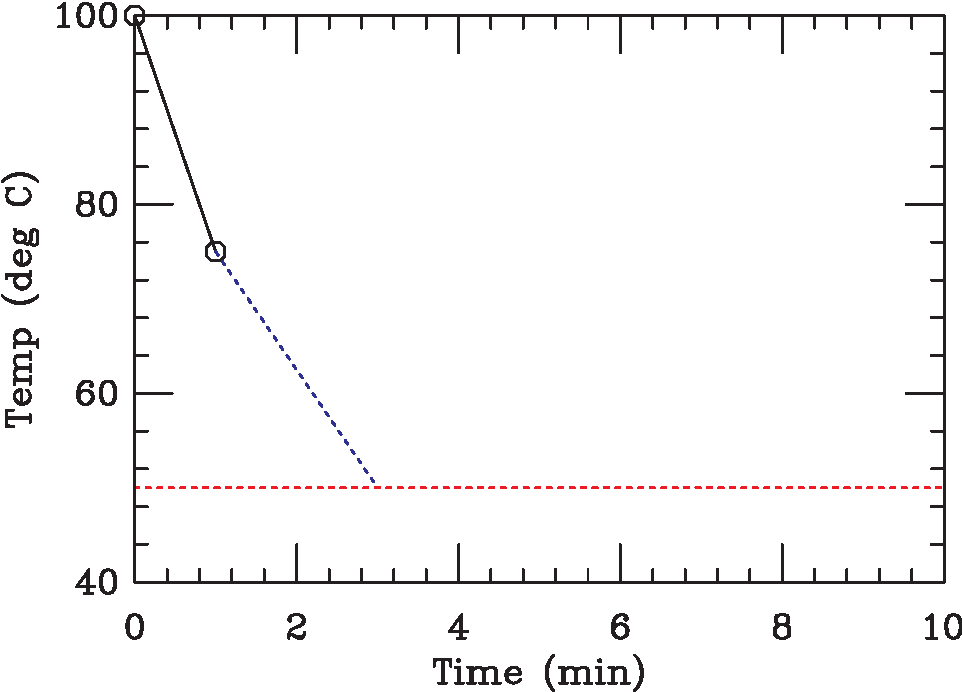
\includegraphics[width=0.4\textwidth]{fig1-crop.pdf}

\vspace{1in}

Questions 5-8 concern the following graph of two functions on the same set of axes. $\alpha(x)$ is shown as a solid line, $\beta(x)$ is shown as a dashed line, and $\gamma(x)$ is shown as a dotted line.

Each function can be expressed as a Taylor series with small coefficients. Specifically, 

\begin{align*}
\alpha(x) &=& a_0 + a_1 x + \frac{1}{2} a_2 x^2 + \frac{1}{6} a_3 x^3 + ...\\ 
\beta(x) &=& b_0 + b_1 x + \frac{1}{2} b_2 x^2 + \frac{1}{6} b_3 x^3 + ...\\
\gamma(x) &=& c_0 + c_1 x + \frac{1}{2} c_2 x^2 + \frac{1}{6} c_3 x^3 + ...
\end{align*}

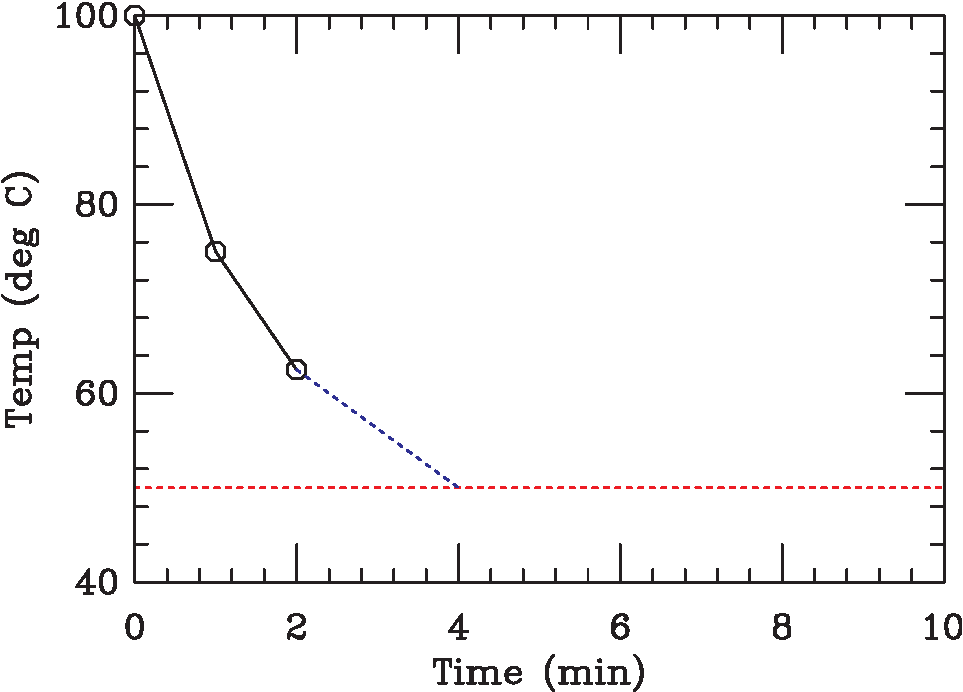
\includegraphics[width=0.4\textwidth]{fig2-crop.pdf}

\item{What is the lowest order $i$ with a nonzero coefficient (``leading order'') for each of $\alpha(x)$, $\beta(x)$, and $\gamma(x)$?}
\vspace{1in}

\item{What is the ratio between the leading-order coefficients for $\alpha(x)$ and $\beta(x)$? (An approximate answer is acceptable.)}
\vspace{1in}

\item{Why are the graphs of all of these functions straight lines on the left-hand side of the graph?}
\vspace{1in}

\item{Why do the graphs of all of these functions begin to curve on the right-hand side of the graph?}
\vspace{1in}



\item{The Taylor series for $\sin(x)$ is $$\sin(x) = x - \frac{1}{6}x^3 + \frac{1}{120}x^5 - ...$$

If you use the small-angle approximation $\sin(x) \approx x$ to calculate $\sin(0.1)$, about how big is the error in the approximation? (You may give just the order of magnitude, for instance, ``${\rm err} \approx 10^{-5}$''.)}

\vspace{1in}


\item{I need one liter of paint to paint a square that is five meters on a side. How many liters of paint do I need to paint a square that is ten meters on a side?}

\vspace{1in}

Questions 11-13 concern the following:

Roughly speaking, the amount of metabolic heat an animal generates is proportional to its volume, while the amount of heat that it loses through its skin is proportional to its surface area. Consider two very similar animals, Animal A and Animal B.
They have identical shapes, identical anatomy, identical anatomy, etc.; the only difference is that Animal B is twice as long, twice as tall, and twice as wide as Animal A. Perhaps Animal A is a small species of deer, while Animal B is a large 
species of deer.



\item{What is the ratio of the heat generated by Animal B to the heat generated by Animal A?}

\vspace{1in}

\item{What is the ratio of the heat lost by Animal B to the heat lost by Animal A?}
\vspace{1in}


\item{Which animal would be more suited to life in a cold climate?}
\vspace{1in}


\end{enumerate}
\end{document}
